\section{Introducción}

% Descripción del proyecto

\begin{frame}{Descripción del proyecto (1/3)}

\begin{itemize}
\item Cátedra Universidad Carlos III - SENER.
\item Desarrollo de un nanosatélite universitario (Proyecto MARTÍN-LARA).
\item Tomar fotografías de la Tierra y estudiar los efectos de la radiación en componentes electrónicos.
\item Filosofía \emph{NewSpace}: Colonizar el espacio con nanosatélites y ofrecer nuevos servicios.
\end{itemize}

\end{frame}


\begin{frame}{Descripción del proyecto (2/3)}

\begin{figure}[h]
\centering
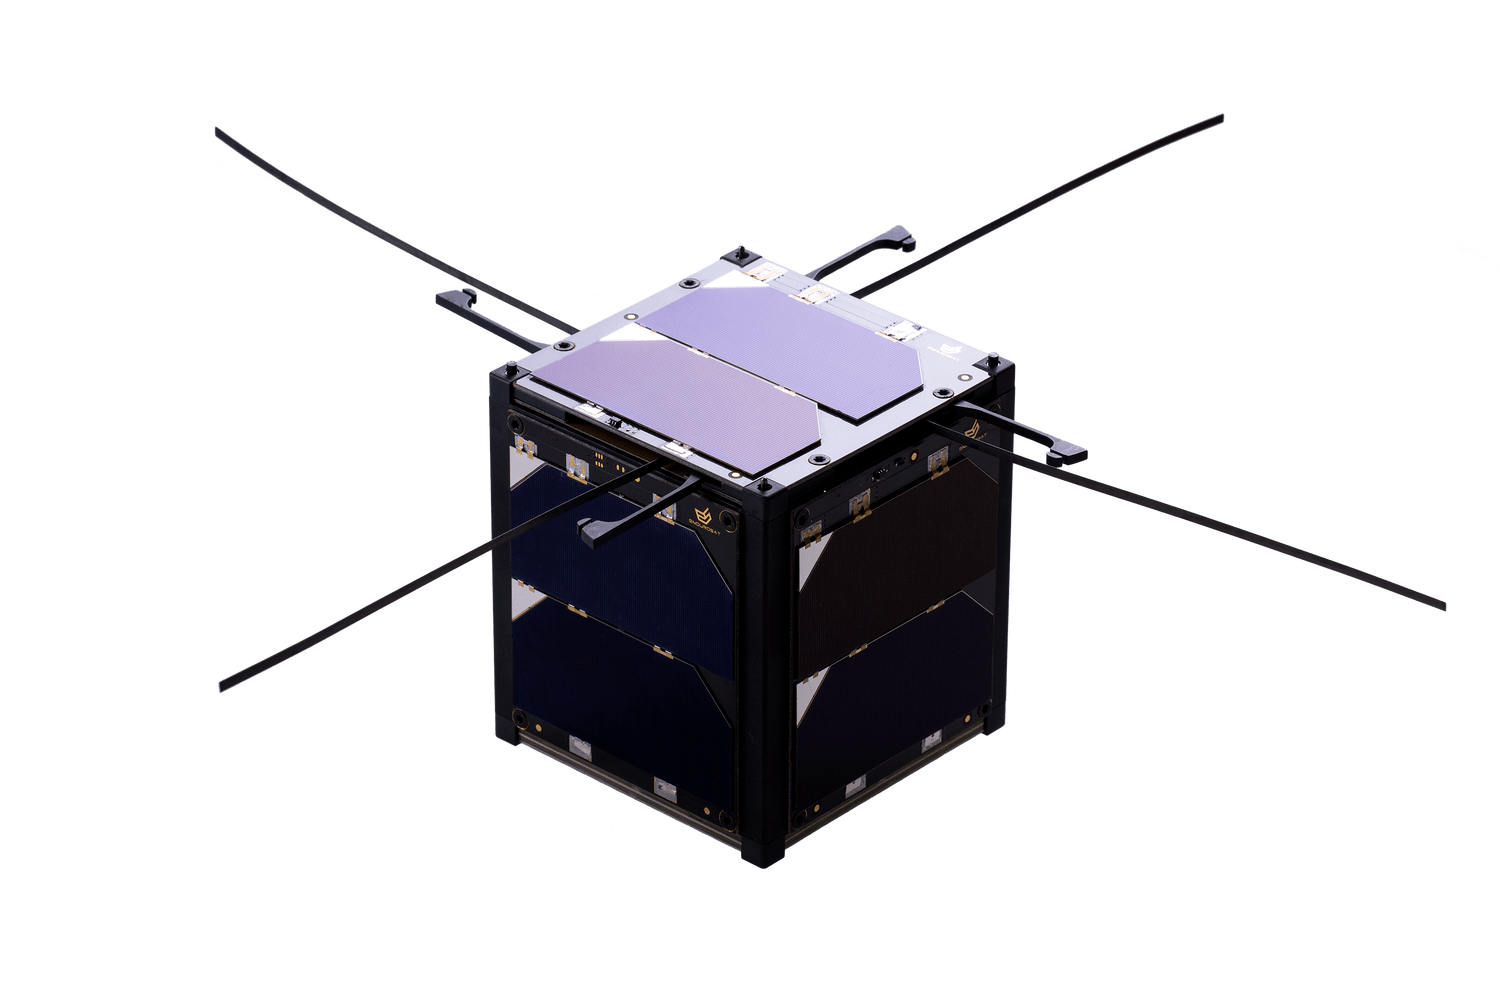
\includegraphics[width=0.4\textwidth]{cubesat}
\caption{\emph{CubeSat}. [Fuente: \texttt{https://satsearch.co/}]}
\end{figure}

Estándar \emph{CubeSat}:

\begin{itemize}
\item Desarrollar nanosatélites en aulas universitarias.
\item Restricciones de dimensiones ($10\times10\times10$ $cm$) y masa ($1.33$ $kg$).
\item Múltiples aplicaciones: observación de la Tierra, comunicaciones, IoT.
\end{itemize}

\end{frame}


\begin{frame}{Descripción del proyecto (3/3)}

\begin{columns}

\column{0.5\textwidth}
\vfill
La mayoría de estas misiones se componen de:

\begin{itemize}
\item Onboard Software (OBSW).
\item Ground System (GS).
\end{itemize}

\vspace{.1in}
Comunicación permanente mediante \emph{data link}.

\vfill

\column{0.5\textwidth}
\begin{figure}
\centering
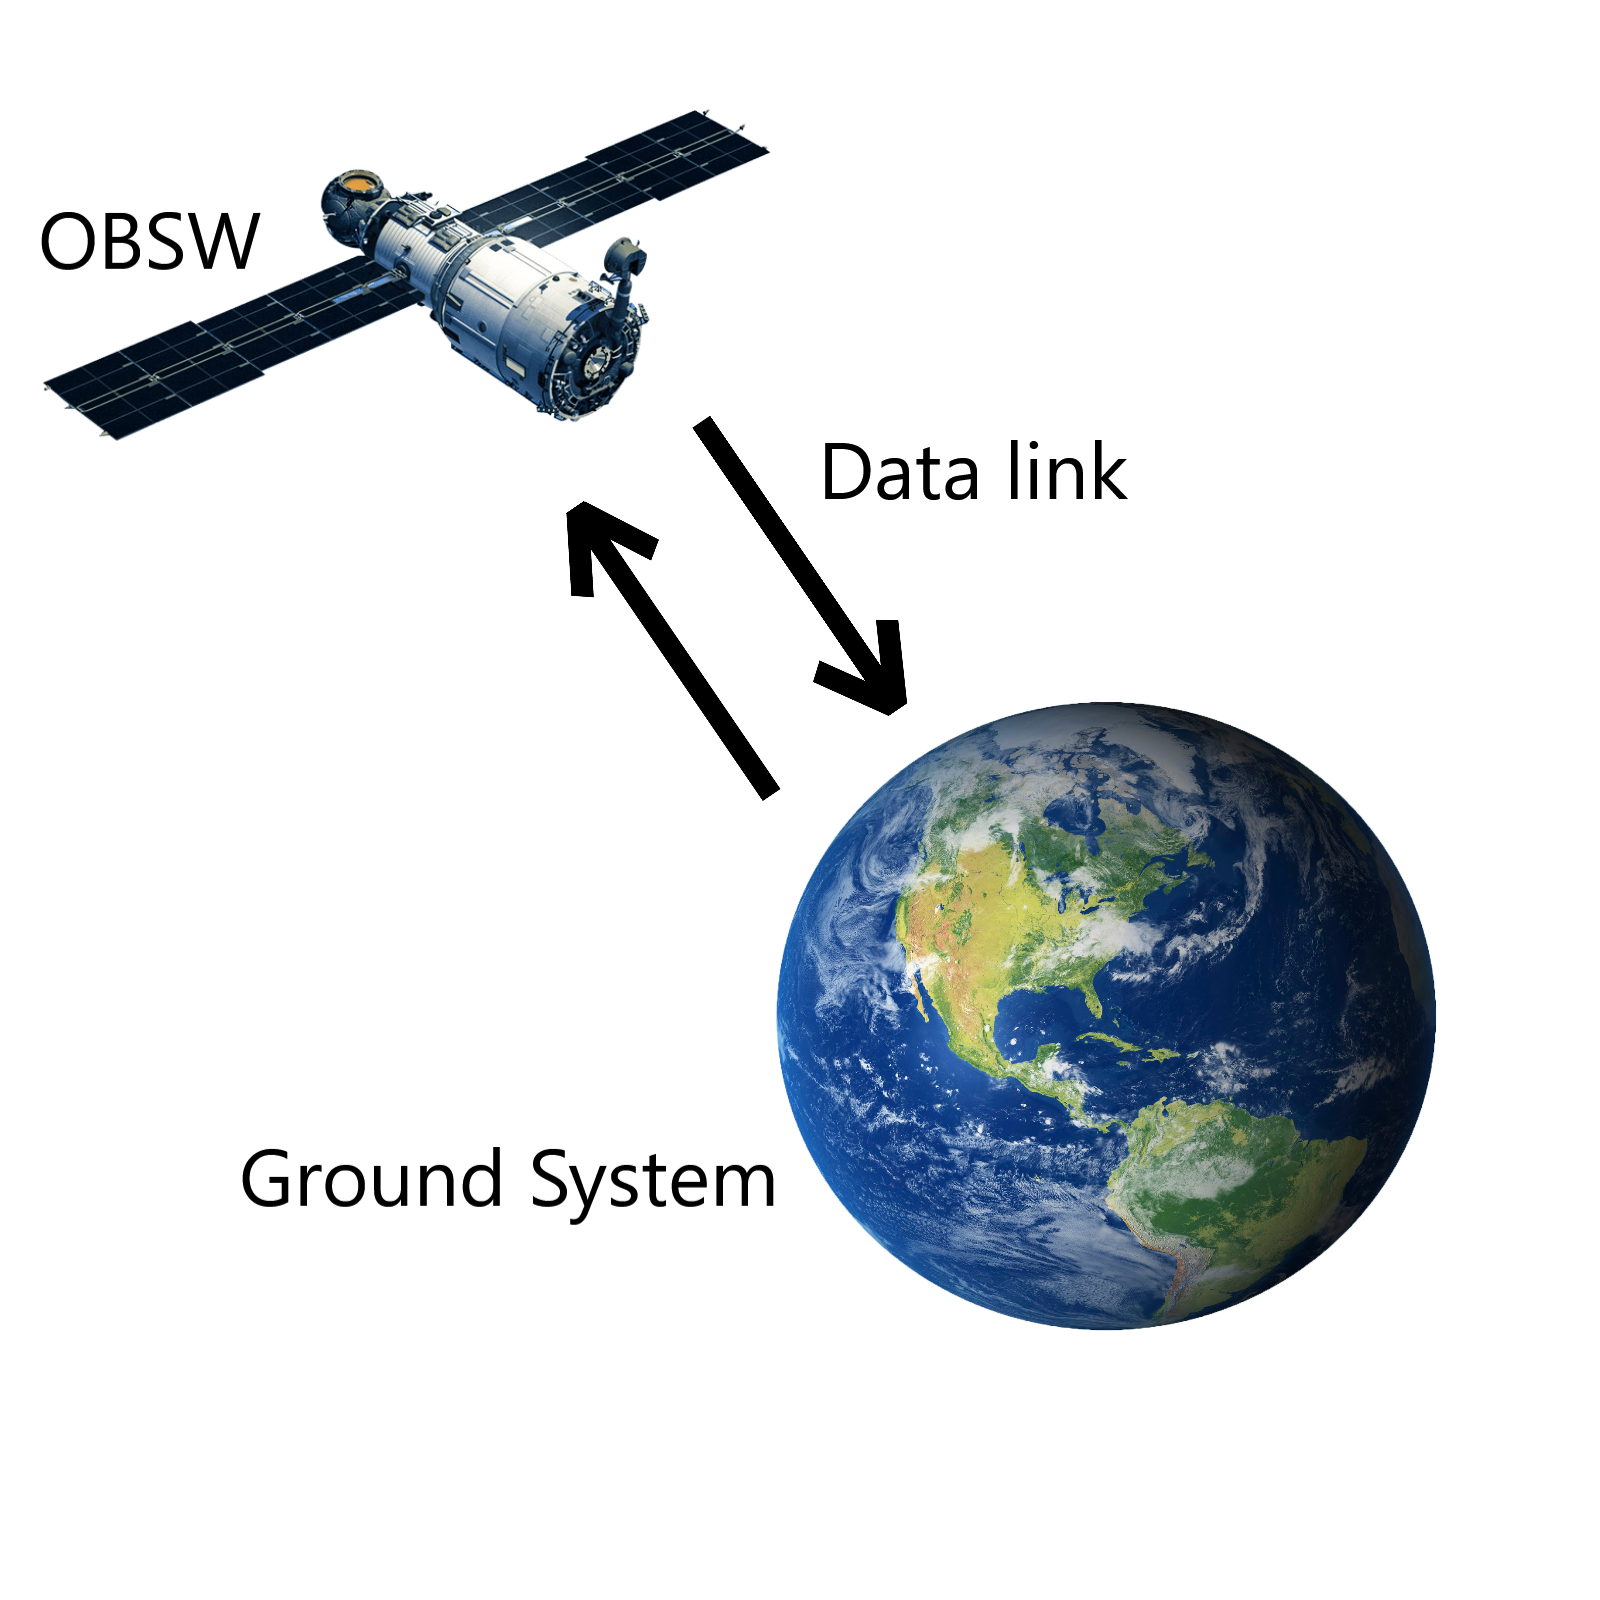
\includegraphics[width=0.9\textwidth]{dataLink}
\caption{\emph{Data link} entre OBSW y GS}
\end{figure}

\end{columns}

\end{frame}


% Motivación

\begin{frame}{Motivación}

El OBSW de estos nanosatélites se caracteriza por:

\begin{itemize}
\item \textbf{Modificación del entorno.} Reciben información del entorno utilizando sensores y modifican su estado con actuadores.
\item \textbf{Sistema crítico.} Ejecutado en un sistema operativo en tiempo real, RTOS. Dos premisas:

	\begin{enumerate}
		\item Ejecutar acciones correctas.
		\item Garantizar plazos de respuesta.
	\end{enumerate}

\end{itemize}

El incumplimiento de una de estas condiciones implica el \alert{fallo total} de la misión.

\end{frame}

% Objetivos

\begin{frame}{Objetivos}

\begin{enumerate}[<+->]
\item \textbf{Definición de la arquitectura del sistema.} Se participará en el diseño de la arquitectura global de la misión.
\item \textbf{Diseño e implementación del simulador térmico.} Definición, diseño e implementación de los diferentes componentes térmicos del sistema.
\item \textbf{Diseño e implementación del módulo de telemetría.} Definición e implementación de los paquetes transmitidos entre diferentes componentes del sistema.
\end{enumerate}

\end{frame}